\section{Reverse-Engineering the App}\label{sec:5}
To further understand the communication between the drone and its app, we used \textit{Frida}, a dynamic instrumentation toolkit, installed on a rooted Android smartphone. This setup allowed us to intercept and analyze the classes, methods, and parameters used by the app while it communicated with the drone.

Using \textit{Frida}, we traced the execution of the app’s methods by running the following command:

\begin{lstlisting}[language=bash]
  frida-trace -U -j com.cooingdv.*!* KY UFO
\end{lstlisting}

This command targets the execution tree of the package \textit{com.cooingdv}, printing every method executed within this package. For each method, \textit{Frida} provided the following information:
\begin{description}
    \item[$\bullet$] The values of the parameters passed to the method.
    \item[$\bullet$] The methods called within the traced method.
    \item[$\bullet$] The return values of the traced method.
\end{description}
\subsection*{Initial Findings}
Through this analysis, we observed a cyclical execution of two key methods:
\begin{enumerate}
    \item \textbf{com.cooingdv.bl60xmjpeg.UAV:} Likely associated with image processing, given the method name and its inferred functionality of handling video streams from the drone.
    \item \textbf{com.cooingdv.kyufo.FlyController:} The method related to controlling the drone, based on its behavior and naming.
\end{enumerate}
To focus our research, we targeted the \textit{FlyController} class specifically by modifying the class path in the previous \textit{Frida} command to be more specific using "\textit{com.cooingdv.kyufo.FlyController.*!*"}
\subsection*{Key Discovery}
Within the \textit{FlyController} class, we identified a method call to \textit{SocketClient.debugSend}.\\
\begin{figure}[h]
    \centering
    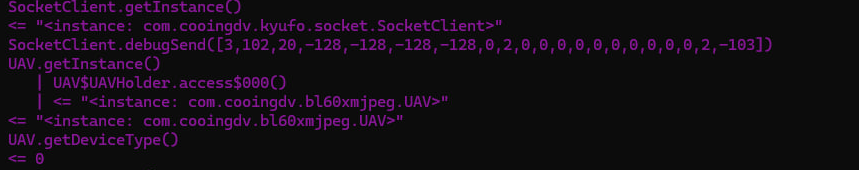
\includegraphics[width=.48\textwidth]{imgs/SocketClientInspect.png}
    \caption{Frida Output}
    \label{fig:name}
\end{figure}
This method had the following 21-byte parameter:\\
3, 102, 20, -128, -128, -128, -128, 0, 2, 0, 0, 0, 0, 0, 0, 0, 0, 0, 0, 2, -103\\
When converted to hexadecimal, the parameter translates to:\\
03 66 14 80 80 80 80 00 02 00 00 00 00 00 00 00 00 00 00 02 99\\
This sequence is nearly identical to the 21-byte packets we intercepted during our traffic analysis:\\
\begin{figure}[h]
    \centering
    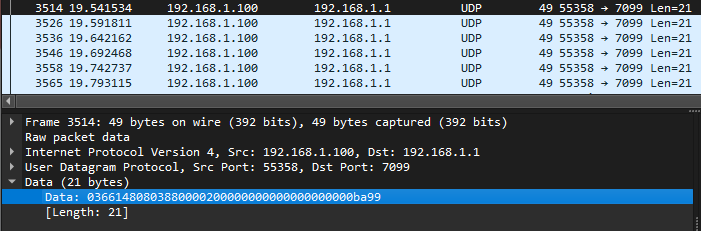
\includegraphics[width=.48\textwidth]{imgs/Packet21B.png}
    \caption{Wireshark Packet Analisys}
    \label{fig:name}
\end{figure}
The similarity strongly suggests that this method is responsible for sending commands to the drone.
\subsection*{FlyController.run}
This method appears to construct and send control packets to the drone based on the state of various flags and control parameters.
The method starts by evaluating a set of boolean flags (\textit{isFastFly}, \textit{isFastDrop}, \textit{isEmergencyStop}, etc.) that represent different states or modes of the drone. These flags are used to calculate a series of integers (\textit{i}, \textit{i2}, \textit{i3}, etc.) through conditional additions. Each flag corresponds to a specific bit position in a byte, and the cumulative value encodes the state.
For example:
\begin{enumerate}
    \item \textbf{isFastFly} adds 1 to the value.
    \item \textbf{isFastDrop} adds 2.
    \item \textbf{isEmergencyStop} adds 4, and so on.
\end{enumerate}
This encoding creates a compact representation of the drone's operational modes in a single byte.\\
Several control parameters (\textit{controlTurn}, \textit{controlAccelerator}, \textit{controlByte1}, \textit{controlByte2}) are validated to ensure they stay within acceptable bounds. For instance:
\begin{enumerate}
    \item \textbf{controlTurn} is clamped between 1 and 255.
    \item \textbf{controlAccelerator} is set to 0 if its value equals 1.
    \item \textbf{}Similar bounds checks are applied to controlByte1 and controlByte2.
\end{enumerate}
This ensures that only valid values are transmitted to the drone, preventing unexpected behavior.

The packet is then costructed using the following structure:
\begin{lstlisting}[language=Java, caption=Packet structure]
  Byte[] bArr = {
  3,
  102,
  20,
  controlByte1,
  controlByte2,
  controlAccelerator,
  controlTurn,
  i9,
  i10,
  0,
  0,
  0,
  0,
  0,
  0,
  0,
  0,
  0,
  0,
  XORControl,
  -103
};
\end{lstlisting}

\begin{lstlisting}[language=Python, caption=XORControl]
  XORControl = i9 ^ 
               {[(controlByte1 ^ 
                    controlByte2) ^ 
                  controlAccelerator] ^ 
                controlTurn} ^ 
               (i10 & 255)
\end{lstlisting}

Finally, the constructed packet is transmitted using either the \textbf{UAV} instance (for active drones) or the \textbf{SocketClient} instance.



\subsection*{Heartbeat mechanism}
The heartbeat mechanism is a crucial periodic signal used to ensure continuous connectivity between the remote controller (RC) and the drone. It serves as a monitoring system, confirming the availability and responsiveness of both components. In essence, the heartbeat mechanism allows the RC and the drone to periodically verify that the other is still reachable and functioning as expected.
%Heartbeat from the Remote Controller

The RC sends a specific 2-byte packet as its heartbeat message. This packet is consistent and unchanging, comprising the following bytes:
\textit{0101}.

This packet is sent at regular intervals of 1000 ms, maintaining the connection between the RC and the drone.
\begin{lstlisting}[language=Java, basicstyle=\small, caption=Heartbeat mechanism] %% codice Heartbeat.run leggermente modificato rispetto all'originale perchè altrimenti non stava nella colonna
public void startUdpTask() {
    UdpComm udpComm = UdpComm.getInstance(
                        "192.168.1.1", 
                        7099);
                                           
    ...// code omitted
    
    Timer timer = new Timer();
    this.netSendTimer = timer;
    timer.schedule(new HeartBeatTask(), 
                    0L, 
                    1000L);
}
    
private class HeartBeatTask 
            extends TimerTask {
    private HeartBeatTask() {
    }

    @Override
    public void run() {
        byte[] beat = new byte[]{1, 1}
        SocketClient.this.debugSend(beat); 
    }
}
\end{lstlisting}